\documentclass{standalone}
\usepackage{tikz}
\usetikzlibrary{patterns, positioning}


\begin{document}
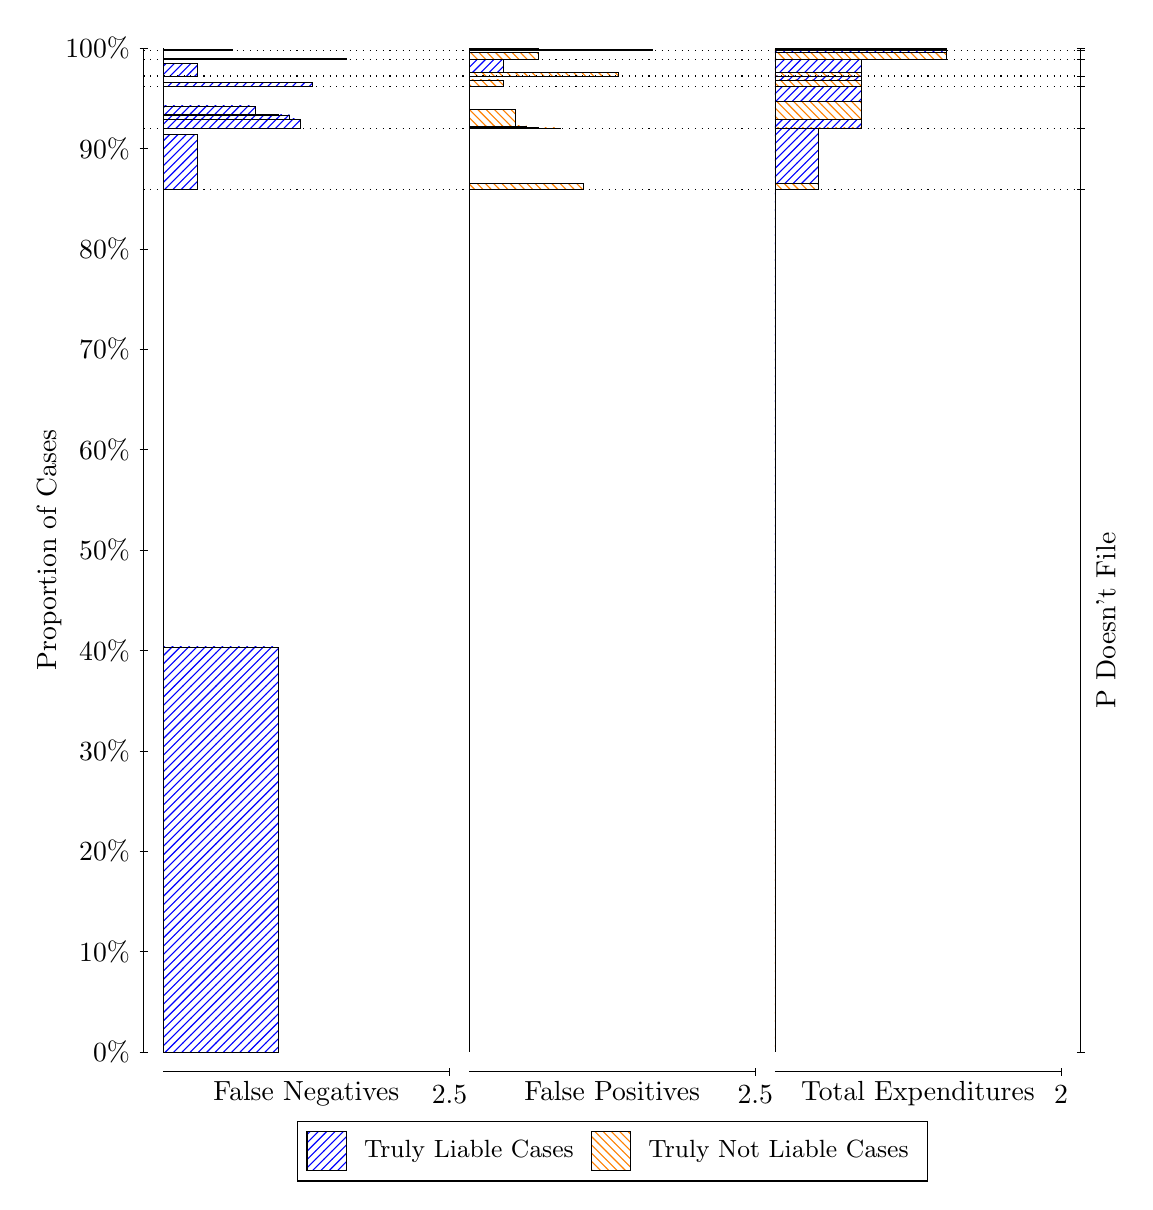
\begin{tikzpicture}
\draw[black, very thin] (1.5,1.75) -- (1.5,14.5);
\node[rotate=90, text=black, anchor=center] at (0.3, 8.125) {Proportion of Cases};
\draw[black, very thin] (1.45,1.75) -- (1.55,1.75);
\node[text=black, anchor=east] at (1.45, 1.75) {0\%};
\draw[black, very thin] (1.45,3.025) -- (1.55,3.025);
\node[text=black, anchor=east] at (1.45, 3.025) {10\%};
\draw[black, very thin] (1.45,4.3) -- (1.55,4.3);
\node[text=black, anchor=east] at (1.45, 4.3) {20\%};
\draw[black, very thin] (1.45,5.575) -- (1.55,5.575);
\node[text=black, anchor=east] at (1.45, 5.575) {30\%};
\draw[black, very thin] (1.45,6.85) -- (1.55,6.85);
\node[text=black, anchor=east] at (1.45, 6.85) {40\%};
\draw[black, very thin] (1.45,8.125) -- (1.55,8.125);
\node[text=black, anchor=east] at (1.45, 8.125) {50\%};
\draw[black, very thin] (1.45,9.4) -- (1.55,9.4);
\node[text=black, anchor=east] at (1.45, 9.4) {60\%};
\draw[black, very thin] (1.45,10.675) -- (1.55,10.675);
\node[text=black, anchor=east] at (1.45, 10.675) {70\%};
\draw[black, very thin] (1.45,11.95) -- (1.55,11.95);
\node[text=black, anchor=east] at (1.45, 11.95) {80\%};
\draw[black, very thin] (1.45,13.225) -- (1.55,13.225);
\node[text=black, anchor=east] at (1.45, 13.225) {90\%};
\draw[black, very thin] (1.45,14.5) -- (1.55,14.5);
\node[text=black, anchor=east] at (1.45, 14.5) {100\%};

\draw[black, very thin] (13.4,1.75) -- (13.4,14.5);
\draw[black, very thin] (13.35,1.75) -- (13.45,1.75);
\node[anchor=west] at (13.35, 1.75) {};
\draw[black, very thin] (13.35,12.709) -- (13.45,12.709);
\node[anchor=west] at (13.35, 12.709) {};
\draw[black, very thin] (13.35,13.475) -- (13.45,13.475);
\node[anchor=west] at (13.35, 13.475) {};
\draw[black, very thin] (13.35,14.012) -- (13.45,14.012);
\node[anchor=west] at (13.35, 14.012) {};
\draw[black, very thin] (13.35,14.145) -- (13.45,14.145);
\node[anchor=west] at (13.35, 14.145) {};
\draw[black, very thin] (13.35,14.351) -- (13.45,14.351);
\node[anchor=west] at (13.35, 14.351) {};
\draw[black, very thin] (13.35,14.469) -- (13.45,14.469);
\node[anchor=west] at (13.35, 14.469) {};
\draw[black, very thin] (13.35,14.5) -- (13.45,14.5);
\node[anchor=west] at (13.35, 14.5) {};

\draw[black, very thin, pattern color=blue, pattern=north east lines] (1.75,1.75) rectangle (3.2033,6.8955);
\draw[black, very thin, pattern color=orange, pattern=north west lines] (1.75,6.8955) rectangle (1.75,12.709);
\draw[black, very thin, pattern color=blue, pattern=north east lines] (1.75,12.709) rectangle (2.186,13.403);
\draw[black, very thin, pattern color=orange, pattern=north west lines] (1.75,13.403) rectangle (1.75,13.475);
\draw[black, very thin, pattern color=blue, pattern=north east lines] (1.75,13.475) rectangle (3.494,13.599);
\draw[black, very thin, pattern color=blue, pattern=north east lines] (1.75,13.599) rectangle (3.3487,13.652);
\draw[black, very thin, pattern color=blue, pattern=north east lines] (1.75,13.652) rectangle (3.2033,13.659);
\draw[black, very thin, pattern color=blue, pattern=north east lines] (1.75,13.659) rectangle (2.9127,13.764);
\draw[black, very thin, pattern color=orange, pattern=north west lines] (1.75,13.764) rectangle (1.75,14.012);
\draw[black, very thin, pattern color=blue, pattern=north east lines] (1.75,14.012) rectangle (3.6393,14.06);
\draw[black, very thin, pattern color=orange, pattern=north west lines] (1.75,14.06) rectangle (1.75,14.145);
\draw[black, very thin, pattern color=blue, pattern=north east lines] (1.75,14.145) rectangle (2.186,14.303);
\draw[black, very thin, pattern color=orange, pattern=north west lines] (1.75,14.303) rectangle (1.75,14.351);
\draw[black, very thin, pattern color=blue, pattern=north east lines] (1.75,14.351) rectangle (4.0753,14.372);
\draw[black, very thin, pattern color=orange, pattern=north west lines] (1.75,14.372) rectangle (1.75,14.469);
\draw[black, very thin, pattern color=blue, pattern=north east lines] (1.75,14.469) rectangle (2.622,14.487);
\draw[black, very thin, pattern color=orange, pattern=north west lines] (1.75,14.487) rectangle (1.75,14.5);
\draw[black, very thin, pattern color=orange, pattern=north west lines] (5.6333,1.75) rectangle (5.6333,7.5633);
\draw[black, very thin, pattern color=blue, pattern=north east lines] (5.6333,7.5633) rectangle (5.6333,12.709);
\draw[black, very thin, pattern color=orange, pattern=north west lines] (5.6333,12.709) rectangle (7.0867,12.781);
\draw[black, very thin, pattern color=blue, pattern=north east lines] (5.6333,12.781) rectangle (5.6333,13.475);
\draw[black, very thin, pattern color=orange, pattern=north west lines] (5.6333,13.475) rectangle (6.796,13.486);
\draw[black, very thin, pattern color=orange, pattern=north west lines] (5.6333,13.486) rectangle (6.5053,13.488);
\draw[black, very thin, pattern color=orange, pattern=north west lines] (5.6333,13.488) rectangle (6.36,13.51);
\draw[black, very thin, pattern color=orange, pattern=north west lines] (5.6333,13.51) rectangle (6.2147,13.723);
\draw[black, very thin, pattern color=blue, pattern=north east lines] (5.6333,13.723) rectangle (5.6333,14.012);
\draw[black, very thin, pattern color=orange, pattern=north west lines] (5.6333,14.012) rectangle (6.0693,14.096);
\draw[black, very thin, pattern color=blue, pattern=north east lines] (5.6333,14.096) rectangle (5.6333,14.145);
\draw[black, very thin, pattern color=orange, pattern=north west lines] (5.6333,14.145) rectangle (7.5227,14.193);
\draw[black, very thin, pattern color=blue, pattern=north east lines] (5.6333,14.193) rectangle (6.0693,14.351);
\draw[black, very thin, pattern color=orange, pattern=north west lines] (5.6333,14.351) rectangle (6.5053,14.447);
\draw[black, very thin, pattern color=blue, pattern=north east lines] (5.6333,14.447) rectangle (5.6333,14.469);
\draw[black, very thin, pattern color=orange, pattern=north west lines] (5.6333,14.469) rectangle (7.9587,14.481);
\draw[black, very thin, pattern color=blue, pattern=north east lines] (5.6333,14.481) rectangle (6.5053,14.5);
\draw[black, very thin, pattern color=orange, pattern=north west lines] (9.5167,1.75) rectangle (9.5167,7.5633);
\draw[black, very thin, pattern color=blue, pattern=north east lines] (9.5167,7.5633) rectangle (9.5167,12.709);
\draw[black, very thin, pattern color=orange, pattern=north west lines] (9.5167,12.709) rectangle (10.062,12.781);
\draw[black, very thin, pattern color=blue, pattern=north east lines] (9.5167,12.781) rectangle (10.062,13.475);
\draw[black, very thin, pattern color=orange, pattern=north west lines] (9.5167,13.475) rectangle (10.607,13.486);
\draw[black, very thin, pattern color=blue, pattern=north east lines] (9.5167,13.486) rectangle (10.607,13.59);
\draw[black, very thin, pattern color=orange, pattern=north west lines] (9.5167,13.59) rectangle (10.607,13.827);
\draw[black, very thin, pattern color=blue, pattern=north east lines] (9.5167,13.827) rectangle (10.607,14.012);
\draw[black, very thin, pattern color=orange, pattern=north west lines] (9.5167,14.012) rectangle (10.607,14.096);
\draw[black, very thin, pattern color=blue, pattern=north east lines] (9.5167,14.096) rectangle (10.607,14.145);
\draw[black, very thin, pattern color=orange, pattern=north west lines] (9.5167,14.145) rectangle (10.607,14.193);
\draw[black, very thin, pattern color=blue, pattern=north east lines] (9.5167,14.193) rectangle (10.607,14.351);
\draw[black, very thin, pattern color=orange, pattern=north west lines] (9.5167,14.351) rectangle (11.697,14.447);
\draw[black, very thin, pattern color=blue, pattern=north east lines] (9.5167,14.447) rectangle (11.697,14.469);
\draw[black, very thin, pattern color=orange, pattern=north west lines] (9.5167,14.469) rectangle (11.697,14.481);
\draw[black, very thin, pattern color=blue, pattern=north east lines] (9.5167,14.481) rectangle (11.697,14.5);
\draw[black, dotted] (1.5,12.709) -- (13.4,12.709);
\draw[black, dotted] (1.5,13.475) -- (13.4,13.475);
\draw[black, dotted] (1.5,14.012) -- (13.4,14.012);
\draw[black, dotted] (1.5,14.145) -- (13.4,14.145);
\draw[black, dotted] (1.5,14.351) -- (13.4,14.351);
\draw[black, dotted] (1.5,14.469) -- (13.4,14.469);
\draw[black, very thin] (1.75,1.5) -- (5.3833,1.5);
\node[text=black, anchor=north] at (3.5667, 1.5) {False Negatives};
\draw[black, very thin] (5.3833,1.45) -- (5.3833,1.55);
\node[text=black, anchor=north] at (5.3833, 1.45) {2.5};

\draw[black, very thin] (5.6333,1.5) -- (9.2667,1.5);
\node[text=black, anchor=north] at (7.45, 1.5) {False Positives};
\draw[black, very thin] (9.2667,1.45) -- (9.2667,1.55);
\node[text=black, anchor=north] at (9.2667, 1.45) {2.5};

\draw[black, very thin] (9.5167,1.5) -- (13.15,1.5);
\node[text=black, anchor=north] at (11.333, 1.5) {Total Expenditures};
\draw[black, very thin] (13.15,1.45) -- (13.15,1.55);
\node[text=black, anchor=north] at (13.15, 1.45) {2};

\node[text=black, centered, rotate=90] at (13.72, 7.2294) {P Doesn't File};







\draw (7.449999999999999,1.5) node[draw=none] (baseCoordinate) {};
\begin{scope}[align=center]
        \matrix[scale=0.5, draw=black, below=0.5cm of baseCoordinate, nodes={draw}, column sep=0.1cm]{
            \node[rectangle, draw, minimum width=0.5cm, minimum height=0.5cm, pattern color=blue, pattern=north east lines] {}; &
            \node[draw=none, font=\small, text=black] (B) {Truly Liable Cases}; &
            \node[rectangle, draw, minimum width=0.5cm, minimum height=0.5cm, pattern color=orange, pattern=north west lines] {}; &
            \node[draw=none, font=\small, text=black] (B) {Truly Not Liable Cases}; \\
            };
\end{scope}

\end{tikzpicture}
\end{document}